\section{Overview and framework}

In this section, we introduce core term definitions and outline the two key issues in estimating the parameters of compact material models, and our techniques to address these challenges (summary functions and Bayesian inference via Monte Carlo sampling).

\subsection{Definitions}

Given a target image $\target$ of a material sample (typically a photograph under known illumination, such as flash), our goal is to estimate the vector of material parameters $\btheta$.

To accomplish this, the first component we will need is a forward evaluator (model) $f(\btheta, \bz)$ which computes a simulated (synthetic) image $\synth$. Here we also consider a vector of random parameters $\bz$ (for example, uniform or normal-distributed); these are essentially controlling the features of the image that have no impact on its ``perceived appearance'' but have significant impact on the numerical values of the pixels; for example, the placement of bumps or scratches. We will require the derivatives of $f$ with respect to $\btheta$.

Therefore, our goal is to find $\btheta$ such that $\synth$ has similar appearance to $\target$, abstracting away from the randomness of $\bz$:
\begin{equation}
	\mbox{find} \ \btheta \ \mbox{s.t.} \ \target \approx f(\btheta, \bz),
\end{equation}
where $\approx$ is a yet unspecified ``appearance match'' relationship.


\subsection{Key challenges}

{\bf Measuring appearance match:} For given material parameters, we can easily evaluate the forward model to predict a synthetic image $\synth$. However, it is not obvious how we can compare it to the target image $\target$ effectively. We clearly cannot use a simplistic image difference metric such as the L2 or L1 norms, because the features (bumps, scratches, flakes, yarns, etc.) in the images will generally not be at matching locations, even if the two images represent the same material appearance. An example if shown in figure \ref{fig:syn1}: each row shows two images of a material with the same parameters $\btheta$ but different random vector $\bz$. The L2 norm of the difference between these image pairs can be large and not useful for optimization.

\begin{figure}[t]
	\addtolength{\tabcolsep}{-3.5pt}
	\begin{tabular}{cc}
		
\includegraphics[width=0.49\columnwidth]{results/bump/syn_comp/bump04rd1.png} &
		
\includegraphics[width=0.49\columnwidth]{results/bump/syn_comp/bump04rd2.png} \\
		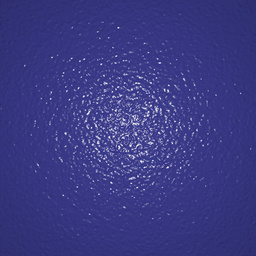
\includegraphics[width=0.49\columnwidth]{results/bump/syn_comp/bump02rd1.png} &
		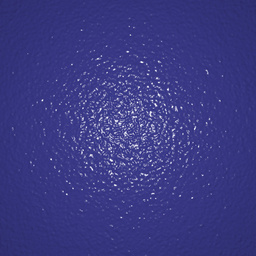
\includegraphics[width=0.49\columnwidth]{results/bump/syn_comp/bump02rd2.png} \\
	\end{tabular}
	\caption{\label{fig:syn1}
		The pairs of images in each row have same the parameters $\btheta$ but with different randomness $\bz$. The pixel-wise L2 norm of the difference between these image pairs can be large and not useful for optimization.
	}
\end{figure}

To address this challenge, we introduce the concept of a \emph{summary function}, which (if chosen well) abstracts away the unimportant differences in the placement of the features, and summarizes the predicted and target images into smaller vectors whose similarity can be judged with simple metrics like L2 distance.

{\bf Similarity structures:} Unless the material model is very simple and/or the target view and lighting are very carefully chosen, it is often not possible to unambiguously determine the full parameter vector from a single image. Instead, there will commonly be an entire region of the parameter space that gives rise to images plausibly matching the target. This may also be due to over-completeness of the parameter space (different settings achieve same look).

Using classical non-linear optimization (or, equivalently, maximum a-posteriori estimation) can often give a good point estimate, matching the target image summary with low error. However, this obscures the fact that many other estimates may also offer good matches to the target, either because the summary function is not powerful enough to distinguish them, or because the difference only shows up under other viewing or lighting conditions. A typical example is the mean scattering angle of the phase function, which is often hard to estimate from a single view; later we will show this and other examples of the similarity structures.

Our proposed solution to this issue is to use Bayesian inference techniques, capable of sampling the space of possible material parameters (the posterior distribution) using Markov chain Monte Carlo methods. This allows a user to both visually inspect the shape of the parameter space (or its low-dimensional projections), as well as click on specific samples and judge the appearance of the result.





